\section{Estudio te\'orico de materiales Bidimensionales}
\subsection{Teor\'ia Funcional de la densidad}
\frame{
	\begin{figure}[!hbt]
		\centering
		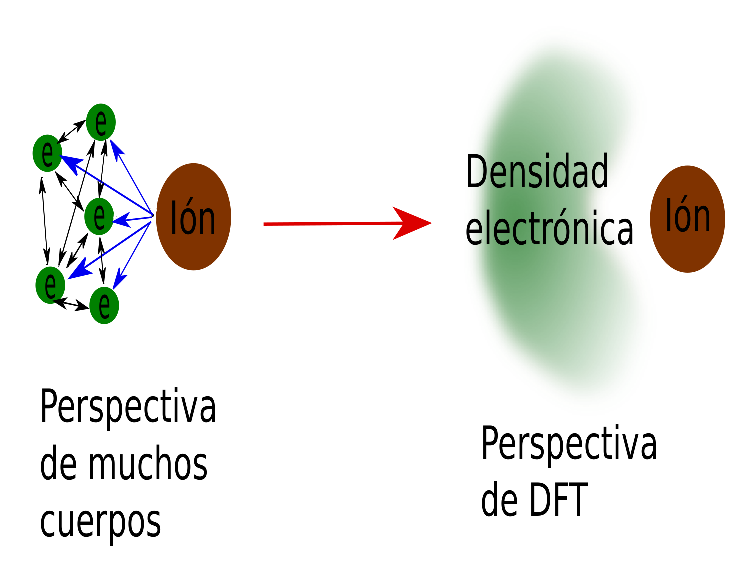
\includegraphics[width=7.0cm,height=7.0cm]{figuras/perspectivaDFT.eps}
		\caption[Perspectiva de la teor\'ia Funcional de la Densidad.]{Idea de la Teor\'ia Funcional de la Densidad.}
		\label{im:dftIdea}
	\end{figure}
}
\frame{
	\frametitle{Ecuaci\'on de Schrödinger de muchos cuerpos}
	La ecuaci\'on fundamental para c\'alculos \textit{ab initio} es la de Schr\"odinger cuyo Hamiltoniano es:
	\begin{multline}
		\hat H = - \frac{\hbar ^2}{2 m_e} \sum_{i} \nabla_{i}^2 - \sum_{i,I} \frac{Z_I e^2}{\vert \pmb{r_i} - \pmb{R_I} \vert}+ \frac{1}{2} \sum_{i \not= j}  \frac{e^2}{|\pmb{r_i} - \pmb{r_j} |}\\
		- \sum_{I} \frac{\hbar^2}{2 M_I} \nabla_I^2 + \frac{1}{2} \sum_{I \not= J} \frac{Z_I Z_J e^2}{|\pmb{R_I}-\pmb{R_J}|}  \label{ec:sh} 
	\end{multline}	
}

\frame{
	\begin{equation}
		\hat H = \hat T + \hat V_{ext} + \hat V_{int}+E_{II} \label{ec:shelectron}
	\end{equation}
    \pause
    \vspace{0.3cm}
    \begin{equation}
    	\hat{T} = \sum_{i} -\frac{1}{2} \nabla_{i}^2 ,\label{ec:shT}
    \end{equation}
    \pause
    \vspace{0.3cm}
    	\begin{equation}
    	\hat{V}_{ext} = \sum_{i,I} V_I (|\pmb{r_i}-\pmb{R_I}|), \label{ec:shVex}
    \end{equation}
    \pause
    \vspace{0.3cm}
    	\begin{equation}
    	\hat{V}_{int} = \frac{1}{2} \sum_{i \not= j} \frac{1}{|\pmb{r_i}-\pmb{r_j}|} \label{ec:shVint}
    \end{equation}
}
\frame{
	\frametitle{Definiciones de la densidad y magnetizaci\'on}
	\begin{itemize}
		\item Densidad de electrones:
		\begin{equation}
			n_{s ', s }(\pmb{r})= \delta_{s',s} \sum_{i} \psi_{i,s '}^ {*} (\pmb{r}) n_{i,s}~ \psi_{i,s } (\pmb{r}). \label{ec:denspin}
		\end{equation}
	   \pause
	   \item Magnetizaci\'on:
	   \begin{equation}
	   	\pmb{m} (\pmb{r}) = - \mu_{B} \sum_{s,s '} \pmb{\sigma}_{s,s'}~ n_{s ', s }(\pmb{r}) , \label{ec:magn}
	   \end{equation}
	\end{itemize}
}
\begin{comment}


\frame{
	\frametitle{Componentes de la magnetizaci\'on}
	\begin{subequations} \label{ec:compm}
		\begin{gather}
			m_x (\pmb{r})= -2 ~\mu_{B} ~Re~ n_{\uparrow, \downarrow} (\pmb{r}) \label{ec:compm1}\\
			m_y (\pmb{r})= -2 ~\mu_{B} ~Im~ n_{\uparrow, \downarrow} (\pmb{r}) \label{ec:compm2}\\
			m_z (\pmb{r}) = - \mu_{B} ~[n_{\uparrow, \uparrow} (\pmb{r})- n_{\downarrow, \downarrow} (\pmb{r})] . \label{ec:compm3}
		\end{gather}
	\end{subequations}
}
\end{comment}
\subsubsection{Teoremas de Hohenberg-Kohn}
\frame{
	\frametitle{Primer teorema de Hohenberg-Kohn}
	\begin{figure}[!hbt]
		\centering
		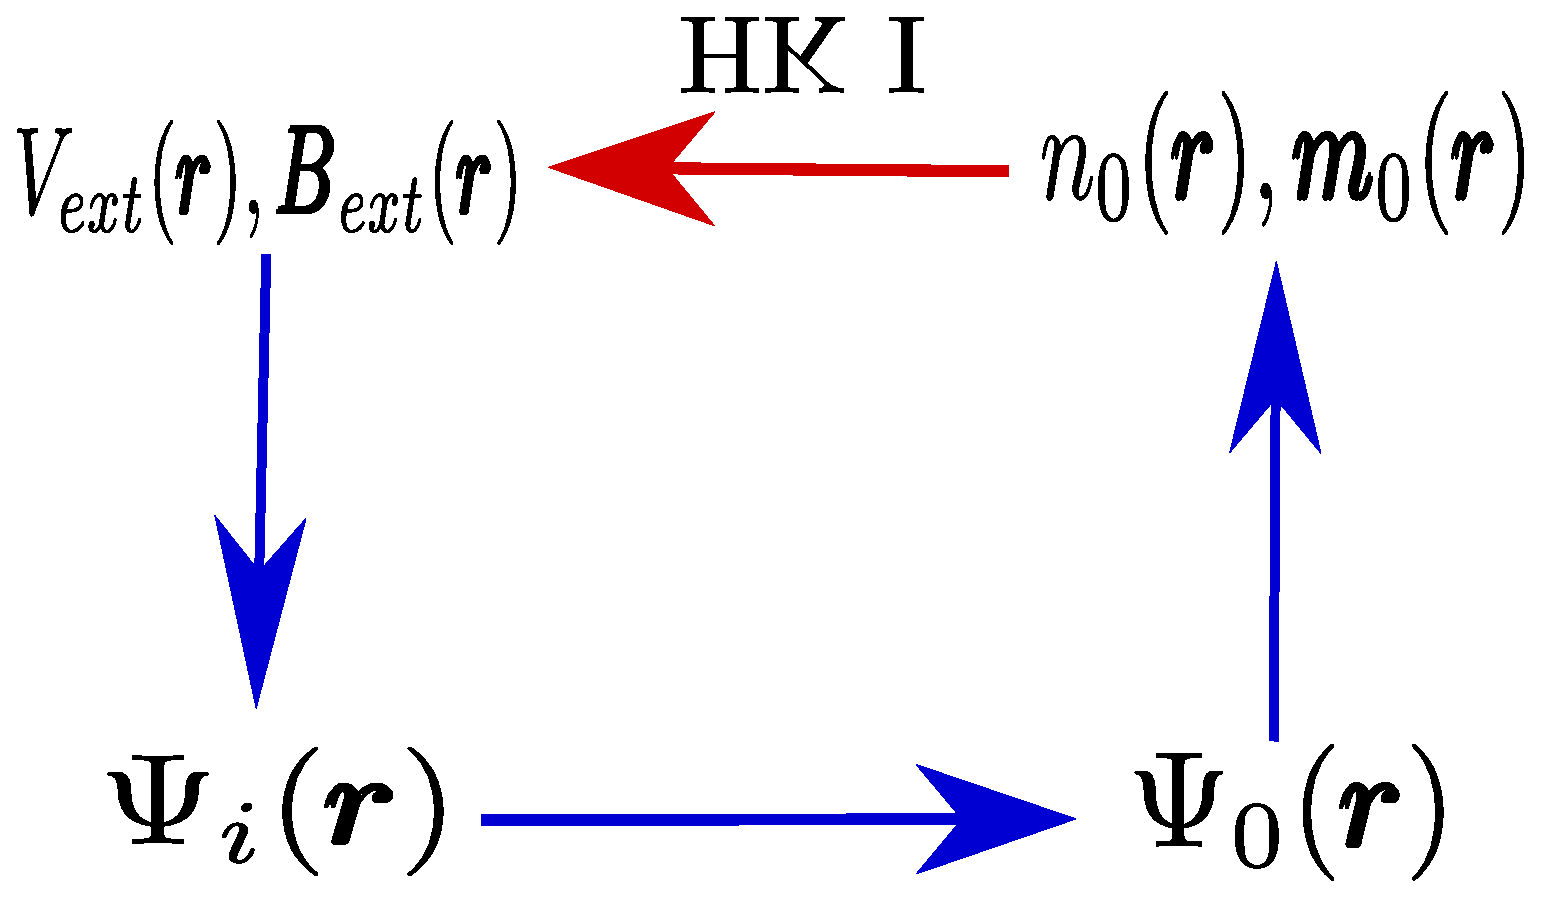
\epsfig{file=figuras/HK1.eps, width=6.0cm,height=5.0cm}
		\caption[Primer teorema de Hohenberg-Kohn]{Representaci\'on esquem\'atica del primer teorema de Hohenberg-Kohn}
		\label{fig:hk1}
	\end{figure}
}
\frame{
  \frametitle{Segundo teorema de Hohenberg-Kohn}
  \begin{equation}
  	E_0 = \min_{n  \to n_0, \pmb{m} \to \pmb{m}_0} E_{V_{ext}, \pmb{B}_{ext}}[n,\pmb{m}]  \label{ec:HKII}.
  \end{equation}
  \pause
  \vspace{0.7cm}
  \begin{equation}
  	E_{V_{ext}, \pmb{B}_{ext}}[n,\pmb{m}]= F[n,\pmb{m}] + \int d \pmb{r} \{V_{ext} (\pmb{r}) n(\pmb{r})+\pmb{B}_{ext} (\pmb{r}) \cdot \pmb{m} (\pmb{r}) \} +E_{II}, \label{ec:funcional}
  \end{equation}
\pause
 \begin{eqnarray}
	F[n,\pmb{m}]&= \langle \Psi_0 [n,\pmb{m}]| \hat{T}+\hat{V}_{int} | \Psi_0 [n,\pmb{m}] \rangle \nonumber \\
	&= T[n,\pmb{m}] + V_{int} [n,\pmb{m}]. \label{ec:funcF}
\end{eqnarray}
}
\subsubsection{Ecuaciones de Kohn-Sham}
\frame{
	\frametitle{Ecuaciones de Kohn-Sham}
	\begin{equation}
		(H_{KS}^s -\epsilon_{i,s})~\psi_{i,s } (\pmb{r}) = 0 \label{ec:ShKS},
	\end{equation}
    \pause
      \vspace{0.3cm}
    \begin{equation}
    	H_{KS}^s = -\frac{1}{2} \nabla^2 + V_{KS}^s (\pmb{r}), \label{ec:HamiltonianoKS}
    \end{equation}
	\pause
	\vspace{0.3cm}
	 \begin{eqnarray}
		V_{KS}^s (\pmb{r}) &=& V_{ext} (\pmb{r})+  \frac{\delta E_{Hartree}}{\delta n_s (\pmb{r})}+  \frac{\delta E_{XC}^s}{\delta n_s (\pmb{r})} \nonumber \\
		&=& V_{ext} (\pmb{r})+ V_{Hartree} (\pmb{r}) + V_{XC}^s (\pmb{r}). \label{ec:potKS} 
	\end{eqnarray}
}
\frame{
	\begin{equation}
		E_{Hartree} = \int d \pmb{r} d \pmb{r'} \frac{n(\pmb{r}) n(\pmb{r'})}{|\pmb{r}-\pmb{r'}|} \label{ec:Hartree}.
	\end{equation}
    	\vspace{0.3cm}
    \begin{equation}
    	E_{XC}^s [n]= \langle \hat{T} \rangle - T_{sp} [n]+\langle \hat{V}_{int} \rangle-E_{Hartree} [n] \label{ec:Exc2},
    \end{equation}
}
\begin{comment}


\subsubsection{Aproximaci\'on PBE}
\frame{
	\frametitle{Aproximaci\'on de gradientes generalizados}
	\begin{multline}
		E_{XC}^{GGA} [n_{\uparrow} (\pmb{r}), n_{\downarrow}(\pmb{r})] = \\ \int d^3 r ~ n(\pmb{r}) \epsilon_{XC} \left(n_{\uparrow} (\pmb{r}), n_{\downarrow}(\pmb{r}), \left|\nabla n_{\uparrow} (\pmb{r}) \right|^2, \left|\nabla n_{\downarrow} (\pmb{r}) \right|^2 \right)  \\
		= \int d^3 r ~ n(\pmb{r}) \epsilon_{X}^{hom} (n) F_{XC} \left(n_{\uparrow} (\pmb{r}), n_{\downarrow}(\pmb{r}), \left|\nabla n_{\uparrow} (\pmb{r}) \right|^2, \left|\nabla n_{\downarrow} (\pmb{r}) \right|^2 \right), \label{ec:funcXCGGA}
	\end{multline}
  \pause
  $ \epsilon_{X}^{hom} (n) = -3k_F / 4\pi $
}
\end{comment}
\frame{
	\frametitle{Ecuaciones de kohn-Sham para el caso no colineal}
	\begin{multline}
		\sum_{s}  \left[-\frac{1}{2} \nabla^2 + V_{ext} (\pmb{r})+ V_{Hartree} (\pmb{r}) + V_{XC} (\pmb{r}) \right] \delta_{s',s}  \phi_{\Lambda} (\pmb{r},s)\\ - \mu_{B} \sum_{s}  [\pmb{B}_{ext} (\pmb{r})+ \pmb{B}_{XC} (\pmb{r}) ] \pmb{\sigma_{s,s'}} \phi_{\Lambda} (\pmb{r},s) = \varepsilon_{\Lambda} \phi_{\Lambda} (\pmb{r},s) , \label{ec:KSnoColl}
	\end{multline}
\pause
 \begin{equation*}
	B_{XCj} (\pmb{r}) = - \frac{\delta E_{XC} [n,\pmb{m}]}{\delta m_j (\pmb{r})} \label{ec:Bxc},
\end{equation*}
}